\documentclass[aspectratio=169]{beamer}

\usepackage{pgfplots}
\usepackage{horaire}
\usepackage{logovdr}
\usepackage{vdr}

\usepgfplotslibrary{groupplots}

\setbeamertemplate{navigation symbols}{}
\setbeamercolor{structure}{fg=marinechum}
\usefonttheme{structurebold}

\begin{document}

\begin{frame}
	\color{marinechum}
	\renewcommand{\contenu}[1]{}
	\frametitle{Formation complémentaire\\\small 28 septembre 2020}

	\begin{minipage}{0.5\textwidth}
		\centering
		\logofvdr[height=4.5cm, fg=structure, fill=grischum!50, ]
	\end{minipage}%
	\begin{minipage}{0.5\textwidth}
		\centering
		\begin{horaire}{450}
		\activite{20}{Accueil des participants}
		\contenu{Feuille de présence}
		\contenu{Attentes des participants}
		\contenu{Objectifs de la journée}
		\activite{15}{État du projet}
		\contenu{Formations des opérateurs}
		\contenu{Formation des médecins}
		\contenu{Formation des autres inhalothérapeutes}
		\contenu{Formulaires}
		\contenu{Matériel}
		\activite{30}{Atelier circuit}
		\activite{60}{Théorie}
		\activite{15}{\it Pause}
		\activite{60}{Atelier paramètres}
		\activite{45}{Contrôle pré utilisation}
		\hline
		\activite{60}{Diner}
		\hline
		\activite{120}{Atelier protocole}
		\activite{40}{Varia}
		\activite{15}{Conclusion}
\end{horaire}

	\end{minipage}

\end{frame}

\frame{
	\frametitle{Contrôle du rapport i:e}
	\centering
	\begin{tikzpicture}[
		cid/.style={
			above=1.35*\ldist,
			align=center,
			font=\tiny
		},
		ie/.style={
			fill=black!15
		},
		index/.style={
			midway,
			below,
			inner
			sep=0,
			font=\tiny,
			scale=0.8
		},
		aug/.style={
			midway,
			above,
			inner
			sep=1mm,
			font=\tiny,
			scale=0.7
		},
		plusmoin/.style={
			below,
			inner sep=1mm,
			font=\tiny,
			%scale=0.7,
		},
		false/.style={
			draw=red,
			cross out
		}
]

\newcommand{\ldist}{7mm}

	\path (0,0) pic [ie, pic text=i] {aknob} 
	node [cid] {FREQUENCE\\DE PERCUSSION};

	\draw [->] (0,0) ++(\ldist, \ldist) -- ++(-2*\ldist, 0) 
	node [index] {$\blacktriangledown$}
	node [aug] {AUGMENTER}
	;

	\path (2.5,0) pic [ie, pic text=e] {aknob}
	node [cid] {RAPPORT\\i/e};

	\draw [<->] (2.5,0) ++(\ldist, -\ldist) 
	node [plusmoin] {+}
	-- ++(0, 2*\ldist) 
	-- ++(-2*\ldist, 0) 

	node [index] {$\blacktriangledown$}
	-- ++(0, -2*\ldist) 
	node [plusmoin] {-}
	node [aug] {}
	;

\end{tikzpicture}

}

\frame{
	\frametitle{Rapport i:e (vue macroscopique)}
	\centering
	\def\iehuit{%
\addplot graphics [
	xmin=0,
	ymin=0,
	xmax=8,
	ymax=60
]}

\begin{tikzpicture}

\begin{groupplot}[
group style={
	group size=1 by 2,
	xlabels at=edge bottom
},
enlargelimits=false,
height=0.46\textheight,
width=\textwidth,
]

\nextgroupplot
\iehuit {img/329-cleaned.jpg};
	\draw <2> [->, ultra thick, bleuclairchum] (axis cs:2.5,0)--(axis cs:2.5,10);

\nextgroupplot
\iehuit{img/629-cleaned.jpg};
	\draw <2> [->, ultra thick, bleuclairchum] (axis cs:4,0)--(axis cs:4,18);

\end{groupplot}
\end{tikzpicture}

}

\frame{
	\frametitle{Rapport i:e (vue microscopique)}
	\centering
	\def\iehuit{%
\addplot graphics [
	xmin=0,
	ymin=0,
	xmax=1,
	ymax=60
]}

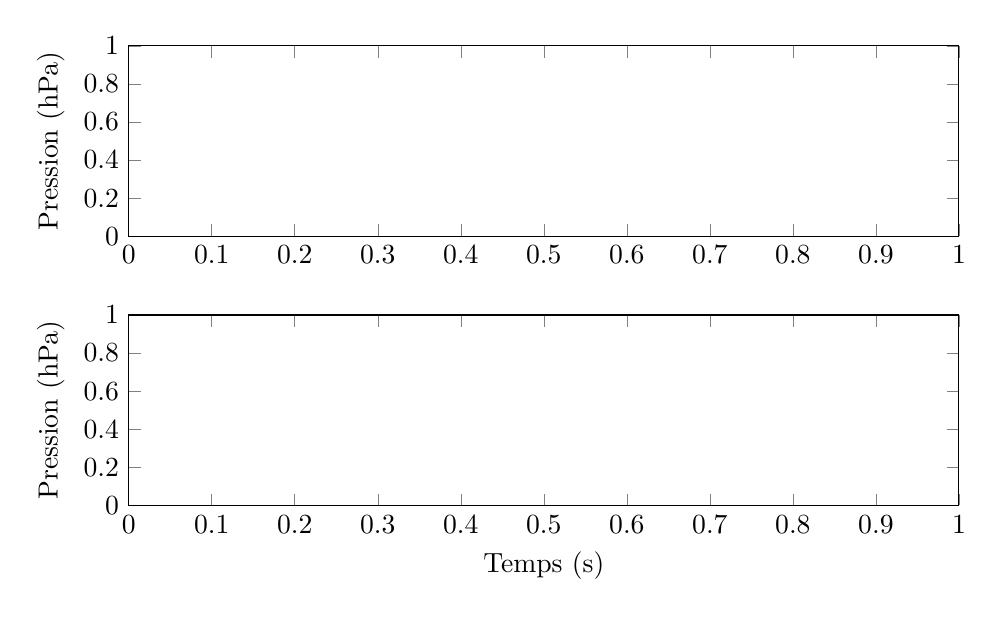
\begin{tikzpicture}

\begin{groupplot}[
		group style={
			group size=1 by 2,
			xlabels at=edge bottom
		},
		enlargelimits=false,
		height=4cm,
		width=\textwidth,
		xtick={0, .25, .5, .75, 1},
		xlabel=Temps (s),
		ylabel=Pression (hPa)
]

\nextgroupplot
\iehuit {img/509.jpg};

\nextgroupplot
\iehuit{img/828.jpg};

\end{groupplot}
\end{tikzpicture}

}

\frame{
	\frametitle{Pressions moyennes inspiratoire et expiratoire}
	\centering
	\newcommand{\pexp}{5}
\newcommand{\pins}{18}
\newcommand{\arrpos}{1.06}
\begin{tikzpicture}[
		pline/.style={
			help lines,
			turquoisechum,
			rounded corners,
			out=0,
			in=180,
			thick
			},
		p/.style={
			circle,
			draw=turquoisechum,
			inner sep=0.5mm,
			thick
			}
	]

	\begin{axis}[
		width=0.65\textwidth,
		name=plot,
		font=\scriptsize,
		try min ticks=6,
		xtick={0,4,8},
		ytick={0,30},
		axis x line=bottom,
		axis y line=middle,
		enlarge y limits={value=0.25, upper},
		enlarge x limits={value=0.05, upper},
		extra y ticks={5, 18},
		extra y tick labels={$P_{ins. moy.}$, $P_{exp. moy.}$},
		extra y tick style={grid=major},
		major grid style={turquoisechum, thick}
		]

		\addplot [
			bleufoncechum,
			restrict x to domain=0:8,
			] table[x=time, y=Pao] {dat/f300.dat};

		\coordinate (D) at (axis cs: \pgfkeysvalueof{/pgfplots/xmax},\pins);
		\coordinate (B) at (axis cs: \pgfkeysvalueof{/pgfplots/xmax},\pexp);

	\end{axis}

	\pic [opacity=0.99, name=mm] at ([xshift=3.2cm, yshift=-.95cm]plot.east) {multimeter};

		\node [grad] (mmg50) at (mmscreen.north west) {50};
		\node [grad] (mmg0) at (mmscreen.south west) {0};
		\draw [pScale]	(mmg0) -- (mmg50) node [grad, left=0.0mm, pos=0.6, inner sep=0mm] {30};

		\node [below, white, align=left, font=\tiny] at (mmscreen.south) {Percussionaire\\Corporation};

	\node [p] (pmi) at (mmPmi) {\pins};
	\node [p] (pme) at (mmPme) {\pexp};

	%\draw [pline] (D) -- ([xshift=4mm]D) |- (pmi);
	%\draw [pline] (B) -- ([xshift=5mm]B) |- (pme);

	\draw [pline] (D) to (pmi);
	\draw [pline] (B) to (pme);
\end{tikzpicture}

}

\frame{
	\frametitle{Séquence des réglages}
	\centering
	\centering
\begin{tikzpicture}

	\pic [name=VDR, black!60, scale=0.8] {vdr};

	\begin{scope}[
		every node/.style={
			color=black,
			}
			]
	\node (1) at (VDR-e) {1};
	\node (2) at (VDR-i) {2};
	\node (3) at (VDR-F) {3};
	\node (4) at (VDR-O) {4};
	\node (5) at (VDR-I) {5};
	\node (6) at (VDR-E) {6};
	\end{scope}

	\begin{scope}[
		every node/.style={
			yshift=8mm,
			align=center,
			scale=0.5
			}
			]
	\node at (VDR-e) {RAPPORT\\i/e};
	\node at (VDR-i) {FREQUENCE\\DE PERCUSSION};
	\node at (VDR-F) {DEPIT\\PULSE};
	\node at (VDR-O) {CPAP\\OSCILLANTE};
	\node at (VDR-I) {TEMPS\\INSPIRATOIRE};
	\node at (VDR-E) {TEMPS\\EXPIRATOIRE};
	\end{scope}

	\begin{scope}[
		every path/.style={
			black,
			opacity=0.80,
			line width=0.7mm,
			->
			},
			]
	\draw [] (1) to (2);
	\draw [bend left=27] (2) to (3);
	\draw [bend left=60] (3) to (4);
	\draw [bend left=45] (4) to (5);
	\draw [bend left=45] (5) to (6);
	\end{scope}

\end{tikzpicture}

}
\end{document}
